\subsection{Estrategia}

Además de los elementos de motivación descritos en la sección anterior, el lenguaje también incluye una serie de elementos de estrategia, en particular la capacidad, los recursos y el curso de acción. Estos se definen como especializaciones de los elementos genéricos de comportamiento y estructura. A continuación, en la figura \ref{tab:EstrategyConcepts}, presentamos un cuadro resumen de los elementos de la capa de estrategia de ArchiMate. El cuadro es una traducción propia basada en la especificación oficial del lenguaje en su versión 3.1.

\newpage
\subsubsection{Elementos de la Estructura}
\begin{table}[h!]
	\begin{center}
		\begin{tabular}{| l | p{6cm} | p{4cm} |} %r c|
			\hline
			Concepto & Descripción & Representación \\ \hline
			
			Recurso
			& 
			Representa los objetos que son controlados o son 
			propiedad de una persona o una organización. 
			& 
			\vspace{0,2mm}	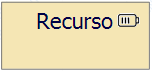
\includegraphics[scale=0.62]{imgs/conceptos/estrategia/Recurso.PNG}	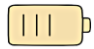
\includegraphics[scale=1.6]{imgs/conceptos/estrategia/imgRecurso.PNG}\\ \hline
			Capacidad 
			& 
			Es la habilidad con la que cuenta una organización, persona o sistema para poder realizar una determinada tarea.
			& \vspace{0,2mm}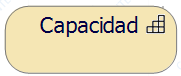
\includegraphics[scale=0.6]{imgs/conceptos/estrategia/Capacidad.PNG}
			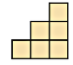
\includegraphics[scale=1.6]{imgs/conceptos/estrategia/imgCapacidad.PNG}
			\\ \hline
			
			Flujo de valor 
			& 
			Representa una secuencia de actividades para crear un resultado general para un cliente, asociado o usuario final.
			& 
			\vspace{0,2mm} 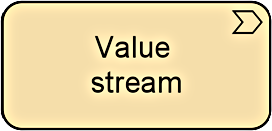
\includegraphics[scale=1]{imgs/conceptos/estrategia/FlujoValor1.png}
			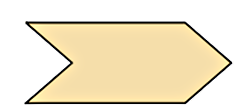
\includegraphics[scale=0.8]{imgs/conceptos/estrategia/FlujoValor2.png}
			\\ \hline
			
			Curso de acción 
			& 
			Representa un plan que organiza las capacidades y habitudes con las que cuenta una empresa, para así poder alcanzar un objetivo o meta. 
			& 
			\vspace{0,2mm} 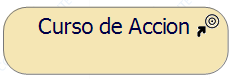
\includegraphics[scale=0.48]{imgs/conceptos/estrategia/CursAcion.PNG}
			
\includegraphics[scale=1.6]{imgs/conceptos/estrategia/imgCursAcion.PNG}
			\\ \hline
		\end{tabular}
		\caption{Elementos de estrategia}
		\label{tab:EstrategyConcepts}
	\end{center}
\end{table}
